\chapter{Исследование и построение решения задачи}
\label{cha:ch_3}

\section{План работы}
Для достижения цели задание было разделено на несколько шагов:

\begin{enumerate}

    \item Подготовка к созданию итоговой модели.
    \begin{enumerate}
        \item Создание простейших симуляций данных со скоплениями.
        \item Выбор архитектуры для сегментации.
        \item Создание образца модели U-net.
        \item Проверка работы U-net на данных симуляций.
    \end{enumerate}

    \item Обработка данных PS1.
    \begin{enumerate}
        \item Загрузка и обработка данных о скоплениях.
        \item Генерация <<патчей>> --- небольших областей неба, на которых будет тренироваться нейросеть.
        \item Загрузка и обработка обзоров неба PanSTARRS1 из области патчей.
        \item Преобразование данных PanSTARRS1 в двумерные матрицы для загрузки в нейросеть.
    \end{enumerate}

    \item Создание модели.
    \begin{enumerate}
        \item Обучение модели, подбор параметров модели (количество слоёв, методы аугментации, размер 
            батча, количество эпох обучения)
        \item Тестирование модели на заранее выбранных данных.
    \end{enumerate}

    \item Постобработка данных и проверка результатов.
    \begin{enumerate}
        \item Преобразование масок сегментации в координаты (детектирование скоплений).
        \item Сравнение полученных скоплений с существующими каталогами.
    \end{enumerate}
\end{enumerate}

\section{Особенности данных}
Матрицы, получающиеся при преобразовании данных из космических 
координат, обычно получаются разреженными и для них приходится использовать значения с плавающей 
точкой. Более того, нужно учитывать точность преобразования и выбирать достаточно детализированное 
разбиение проекции на пиксели изображения, иначе разные объекты могут слиться в один. Угловой 
размер области тоже имеет значение, так как на слишком маленьких частях неба искать такие большие 
объекты, как скопления галактик, бессмысленно.\\


\section{Создание симуляций}
Для создания симуляций использовался простейший алгоритм с использованием генерации случайных 
данных. По предположению данные скоплений можно аппроксимировать равномерным, пуссоновским и 
гауссовым распределениями.
Поэтапно создание симулированных данных выглядит так:

\begin{enumerate}
	\item Равномерным распределением создаём заданное количество скоплений на изображении.
	\item Для каждого скопления выбираем размер и количество объектов из распределения Пуассона.
	\item Для каждого скопления координаты объектов генерируются из распределения Гаусса.
	\item Равномерно генерируются координаты объектов шума.
\end{enumerate}

\begin{figure}[h]
    \center{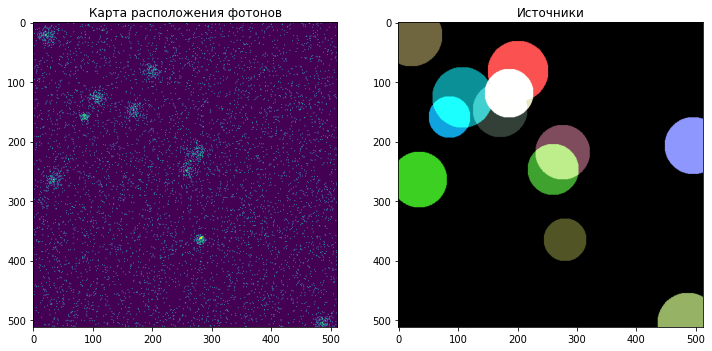
\includegraphics[width=0.7\linewidth]{gen0}}
    \caption{Пример генерации симулированных данных со скоплениями}
\end{figure}


\section{Обработка данных PS1}
Так же, как и в статье \cite{Bonjean}, в качестве списка скоплений будем использовать каталог PSZ2. 
Аналогичным образом будем генерировать патчи для создания тренировочных, валидационных и тестовых 
выборок (в том числе для валидации и тестирования будут выбраны те же пиксели разбиения $n_{side}=2$. 
Патчи выбирались так, чтобы в их окрестности находился хотя бы одно из скоплений нужного каталога. 
После этого в базе данных PS1 (Pan-STARRS1) запрашивался список объектов, подходящих под заданные 
условия. \\

Для каждого объекта из PS1 загружелись следующие данные:
\begin{enumerate}
    \item id объекта.
    \item Координаты объекта.
    \item (filter)PSFFlux - информация о ядре объекта.
    \item (filter)PSFFluxErr - ошибка измерения (filter)PSFFlux.
    \item (filter)KronFlux - информация о полном свете объекта.
    \item (filter)KronFluxErr - ошибка измерения (filter)KronFlux.
\end{enumerate}

Вместо (filter) подставляется одна из букв \{g, r, i, z, y\}, обозначающих фильтр, которым 
обрабатывалась информация об объектах. Таким образом, информация об излучении объекта хранится в 
20 параметрах, включая ошибки.\\

Из-за особенностей данных, некоторые объекты могут повторяться (то есть их координаты полностью 
совпадают). В таких ситуациях нужно провести слияение объектов --- для каждого из параметров 
(filter)PSFFlux и (filter)KronFlux нужно сохранить значение из той строки, где ошибка 
соответствующего измерения будет ниже. Оставшиеся значения ошибок можно либо удалить из данных, 
либо использовать их для аугментации: 
каждый раз при переносе значения какого-либо параметра, прибавлять к нему случайное значение из 
нормального распределения $N(0, (filter)(parameter)Err)$.\\

После того, как будут получены данные для обучения, их нужно из таблиц преобразовать в двухмерные 
матрицы изображений, чтобы создать выборки с количеством каналов, совпадающих с количеством 
исследуемых параметров у объектов. \\

Для примера, таблица с данными для 50 патчей содержит около 10 миллионов объектов. Обработка 
сотни объектов будет длится несколько минут, поэтому необходимо отдельно распараллелить процесс.\\

Для обучения планируется использование параметров (filter)KronFlux, то есть у первой версии 
нейросетевой модели будет 5 входных слоёв. Значения (filter)PSFFlux нужны для того, чтобы заменить 
ими отсутствующие измерения (filter)KronFlux для некоторых объектов.\\

